\documentclass{article}

\usepackage{a4}
\usepackage{setspace}
\usepackage{graphicx}
\usepackage{amsmath}
\usepackage{mhchem}
\usepackage{hyperref}

\setlength{\parindent}{0pt}

\title{A Deeper Understanding of the s-Process:\\
A Ph.D. Oral Qualifier}
\author{by: Jaad A. Tannous\\
Advisor: Prof. Bradley S. Meyer}
\date{}

\begin{document}
\maketitle

\section*{Abstract}
The aim of this document is to provide the committee a quick recap of the s-process, and how I aim to 
contribute to further its understanding. The first section is a brief recap, but granted not a complete 
one, on the s-process. The following four will outline tools being developed, and aspects that are being 
studied. In the last section I will conclude how the project will come together.

\section*{The s-process}
The slow neutron capture process, s-process, is a series of reactions in nuclear astrophysics that is responsible 
for synthesizing half the elements heavier than Iron. It occurs in moderately neutron rich environments and requires 
existing iron as a seed nucleus. The reactions involved are a series of neutron captures and $\beta^{-}$ decays. Heavier 
isotopes will form until one that is $\beta$ unstable is reached, and its decay rate is shorter than the capture rate; as illustrated 
in Fig. 1.

\begin{figure}[!htp]
    \centerline{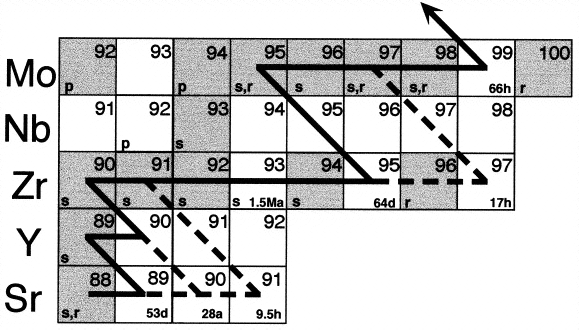
\includegraphics[scale = 0.5]{images/sprocess.png}}
    \caption{A Z-N flow chart illustrating a cut of s-process nucleosynthesis from Strontium up till 
    Molybdenum. The solid line indicates the main path, while the dotted a secondary branch \cite{nic98}.}
\end{figure}

 It is a slow process because the $\beta^{-}$ decays occur on shorter timescales than the next neutron capture. In comparison, 
neutron captures may take days or years, while beta decays can take between seconds and hours.\\

 S-process nucleosynthesis occur in two types of stars; during Thermal Pulsing Asymptotic Giant Branch stars, TP-AGB, and massive stars 
have achieved core Helium burning and beyond. The yield and extent s-process can generate has two major factors. The first being the 
star's capability to generate neutrons. The second being the amount of Iron the star was able to accrete from the cloud it formed from.\\

 The yields and end products generated by TP-AGB stars and massive stars are so different, they are categorized into main branch and weak 
branch s-process. The main branch s-process nucleosynthesis occurs in TP-AGB stars, specifically in low mass stars. It produces heavy 
elements up to Lead in low metallicity stars. In this phase, neutron source is $^{13}C$ created during the third dredge up \cite{kww} and 
produces neutrons via:

\begin{equation*}
\ce{^13C + ^4He -> ^16O + n} 
\end{equation*}

 The weak s-process branch occurs at the end of core Helium and Carbon burning in massive stars. It produces heavy elements up Yttrium.
The element that will supply the neutron is the isotope $^{22}Ne$ via:

\begin{equation*}
    \ce{^22Ne + ^4He -> ^25Mg + n}
\end{equation*}

 Due to low neutron fluxes, $10^{5}$ to $10^{11} cm^{-2}s^{-1}$, the s-process cannot produce the heavy radioactive such as Uranium. 
However, it terminates in a Bismuth, Lead, Polonium loop:

\begin{align*}
    \ce{^209Bi + n &-> ^210Bi + \gamma}\\
    \ce{^210Bi &-> ^210Po + e^- + \bar{\nu_{e}}}\\
    \ce{^210Po &-> ^206Pb + ^4He}\\
    \ce{^206Pb + 3n &-> ^209Pb}\\
    \ce{^209Pb &-> ^209Bi + e^- + \bar{\nu_{e}}}
\end{align*}

\section*{Neutron Exposure}

For a given species 'i' whose only interaction is neutron capture, its total abundance over time is governed by:

\begin{align*}
    \frac{d Y_{i}}{dt} &= -N_{A}\left<\sigma v\right>\rho Y_{i}Y_{n}\\
    \frac{d Y_{i}}{dt} &= -n_{n} \left<\sigma v\right> Y_{i}
\end{align*}

The differential exposure and neutron capture cross-section are respectively given by:
\begin{align*}
    d\tau &= n_{n}v_{T}dt\\
    \sigma_{i} &= \frac{\left<\sigma v\right>}{v_{T}}
\end{align*}

Where $n_{n}$ is the neutron number density and $v_{T}$ is the thermal velocity of neutrons. The first order differential equation 
now becomes

\begin{equation*}
    \frac{d Y_{i}}{d\tau} = -\sigma_{i}Y_{i}
\end{equation*}
And has a solution
\begin{equation*}
    Y_{i}(\tau) = Y_{i}(0)e^{-\sigma_{i}\tau}
\end{equation*}

Realistically, we always have an ensemble of species with unique cross-sections. Such an ensemble requires the introduction  of a 
normalized density of exposures $\rho(\tau)$. The above differential equation has the general solution:

\begin{equation*}
    Y_{i}(\tau) = Y_i(0)\int_{0}^{\infty}\rho(\tau)e^{-\sigma_{i}\tau}d\tau
\end{equation*}

Generally speaking, $\rho(\tau)$ is unknown and must be solved for. An exponential distribution of exposures was suggested \cite{clayton1974s}, 
however it is specific to certain mixing models. With additional mixing processes induced by rotation and magnetic fields, a 
general form for the density of exposures is necessary. Upon closer inspection, we realize that

\begin{equation*}
    \frac{Y_{i}(\tau)}{Y_i(0)} = \int_{0}^{\infty}\rho(\tau)e^{-\sigma_{i}\tau}d\tau = \tilde{\rho}(\sigma_{i})
\end{equation*}

Where $\tilde{\rho}$ is the Laplace transform of the exposure density into cross-section space, which is easily attainable using 
libnucnet \cite{meyer}. The exercise becomes solving for the inverse Laplace transform in post-processing. Formally, the inverse 
Laplace transform is determined by the Bromwich integral:

\begin{equation*}
    \rho(\tau) = \frac{1}{2\pi i} \lim_{T\to\infty}\int_{\gamma - iT}^{\gamma + iT}e^{\sigma_{i}\tau}\tilde{\rho}(\sigma_{i})
\end{equation*}

Which is a line integral in the complex plane. Without having an analytical form for $\tilde{\rho}$, solving the integral with standard 
procedures, such as Cauchy Residue theorem, is quite challenging numerically. To circumvent said challenge, we apply the Gaver-Stehfest 
method \cite{jacquot1983gaver}. In short the method transforms the integral into the real plane and suggests an appropriate discretization. 
Figures 2 and 3 show the method's effectiveness at approximating the inverse, where the analytical forms are known. 
The notebook used to generate the graphs is found \href{https://github.com/jaadt7/gaver_stehfest}{here}.

\begin{figure}[!htp]
    \centerline{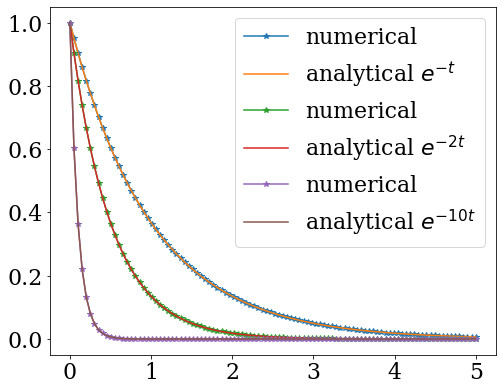
\includegraphics[scale = 0.5]{images/exp_test_1.png}}
    \caption{Testing the Gaver-Stehfest method on decaying exponential functions}
\end{figure}

\begin{figure}[!htp]
    \centerline{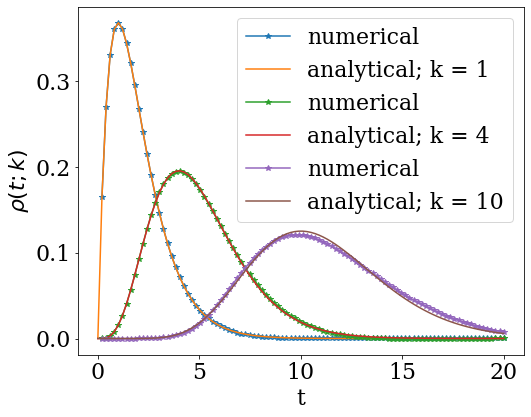
\includegraphics[scale = 0.5]{images/poisson_test.png}}
    \caption{Testing the Gaver-Stehfest method various Poisson distributions}
\end{figure}

\section*{Isomers}
\section*{T and $Y_{e}$ dependent rates}
\section*{Multizone framework development}
\section*{My research}

\singlespacing

\bibliographystyle{apalike}
\bibliography{references.bib}

\end{document}